\chapter{Background}
% 10-20 pages
% This should form the bulk of the interim report. 
% You should consider that your objective here is to produce a near final version of the background section, as it will appear in your final report. 
% All of this material should be re-usable, so it is worth getting it right at this stage of the project.  
% The details of what to include can be found in the Project Report guidelines.

% - Perching Approaches
% - Reinforcment Learning
%   - Traditional
%     - FYP11 - Review Paper - maybe just discuss some findings
%     - Previous Work - done
%     - FYP8 - Human-Level Control through Deep Reinforcment Learning
%     - FYP12/23 - Autonomous Waypoint Navigation
%     - FYP13 - Noise Injection
%   - Apprentiship Reinformcent Learning 
%     - FYP7 - "An Application of Reinformcent Learning to Aerobatic Helicopter Flight (P. Abel 2007)" - done
%   - Demonstration
%     - FYP9 - DeepQ Learning from Demonstration - done
%     - FYP14 - Learning from Imperfect Demonstrations
%     - FYP-16 - Forgetful Experience Replay in Hierechical Reinfrocment Learning from Expert Demonstrations.
%     - FYP17 - Mapless navigation for UAVs via Reinforcement Learning - done
%   - Transfer Learning
%     - FYP10 - Soft Actor-Critic with Inhibitory Networks for Retraining UAV Controllers Faster
%     - FYP18 - Inverse Reinforcement Learning
%   - Learned Skills
%     - FYP-15 - Demonstration Guided Reinforcment Learning with Learned Skills

% Previous Work - Fabian
The aim of this chapter is to provide an extensive review of perching techniques and automated trajectory generation, with particular focus on methods that require minimum simulation interaction.
In order, we will cover various perching approaches, previous work on automated perching and reinforcement learning with demonstrations.

\section{Perching Approaches}

\section{Previous Work}

% Previous Work

Previous work has explored the use of Reinforcement Learning in automatically generating trajectories for drone perching\cite{learnedTetheredPerchingFabian}.
In this approach a Soft Actor Critic algorithm was employed to develop a series of energy optimised trajectories.
The trajectory was divided into three seperate stages.
The initial approach and contact phases used trajectories formulated using analytical solutions.
The Reinformcent Learning aspect was specifically applied for the more complex manuver of flipping the drone beneath the branch.

\todo{diagram for this manuever}
\begin{figure}[htbp]
  \centering
  
\includegraphics[width=0.33\textwidth]{frog.png}
  \caption{TODO}
\label{fig:previous-work-manuever-diagram}
\end{figure}

A Markov Decision Process was defined using observations $o_{t} \in O$ where $o_{t}$ denotes the drone's relative position and $a_{t}$ determines its roll rate.
An experimental baseline provided a potential solution using a constant roll rate.
This method integreated two components of a reward function.
In the initial training stages, the algorithm priotitised conforming to the baseline.
As training progresses, there is a shift in the reward function's focus, increasingly favouring a faster, more energy efficient trajectory.
This shift allows a greater exploration of the parameter space.

\[
R_{1}(s_{t}, a_{t}) = 
\begin{cases} 
I(s_{t}, a_{t}) & \text{for } t \leq t_{I} \\
I(s_{t}, a_{t}) M(t) & \text{else} 
\end{cases}
\]

\[I(s_{t}, a_{t}) = 3 \times 10 ^ 5 \times (0.1 - \min(|s_{\alpha} - s'_{\alpha}|, 0.1)) ^ 4\]
\[M(t) = \frac{t_{\max} - t}{t_{\max} - t_{I}}\]

\[
R_{2}(s_{t}, a_{t}) =
\begin{cases}
  R_{L} + \frac{\Delta X_{target} - 0.005}{l_{r}} \times 50 & \text{for } \frac{d_{target}}{d_{drone}} > 1 \\
  R_{L} + \frac{\Delta X_{branch}}{d_{drone}} \times 100 & \text{else}
\end{cases}
\]

\todo{rephrase this section}
where $s_{\alpha}$ and $s_{\alpha}$ are the roll angel of the current and the baseline state; 
$t_{\max}$ is the maximum time of the simulation; 
$t_{I}$ is the time where the final point should be reacted.
where RL is the reward from the last step dtarget is the distance to the target position; 
ddrone is the size of the drone; 
$\delta$Xtarget and $\delta$Xbranch is the change in the distance made to the final position and to the branch, and lr is the length of the rope.

However this method may constrain the range of possible solutions.
By favouring approaches that resemble the baseline, this could prevent the system from learning novel, potentially more efficient strategies.
Since just roll rate was explored, this limits the range of solutions into 2 dimensions which reduces the computational complexity but may not fully explore paths.
Additioanlly one of the main challenges in the previous work was simulation.
Accurately modelling the dynamics between the tether and the drone presented significant challenges.
Performing training in a real-world setting would be exceptionally difficult, given the extensive number of trials required and the risk of errors causing physical damage to the drone.

There is a need to devise a system capable of efficiently learning from a very limited number of experiments, while ensuring safety of the drone. \\\\

\section{Reinforcement Learning}
% Intro
Reinforcement learning involves an agent that interacts with an environment to gain knowledge and recieve feedback in the form of rewards~\cite{rlIntroSuttonBarlo}.
The agent explores the environment, discovers which actions yield the most reward, and then refines its strategy to produce an optimal policy.
States are a mathematic representation of the environment, and must contain all information required to compute the optimal policy.
Within the particular task of drone perching, this is likely to include coordinate positions along 3 and angles along all axis and the velocities along all axes.
The actions here represent what the drone will execute to solve the problem which for this problem represents the coordinate positions of movement which will represent the trajectory.
The development of Deep Q-Networks combining neural networks with reinforcement learning has proved extremely successful in the Atari Games, a popular benchmark in RL.

\todo{do this diagram and finish the text above}
\begin{figure}[htbp]
  \centering
  
\includegraphics[width=0.33\textwidth]{frog.png}
  \caption{TODO}
\label{fig:rl-intro-drone}
\end{figure}

% FYP11 - Review Paper - maybe just discuss some findings
The problem of trajectory generation for drone perching has a large overlap with UAV navigation.
Therefore when investigating work on reinforcement learning this was a particular area that was focussed on since the objective is largely the same.
In 2022 a review paper\cite{aerialNavReview} on UAV navigation using RL identified 159 papers that use RL to solve UAV navigation challenges.
Within path planning the review described papers based on both mapless and map-based navigation.
A map-based navigation approach uses a representation of the environment, largely including terrain or obstacles.
Within drone perching this would likely relate to s \todo{finish this}

However one of the major limitations of traditional reinforcement learning in this context is the high number of episodes required to train.
This is different to navigation tasks which can be simulated reasonably well. \\\\

% FYP8 Human-Level Control through Deep Reinforcment Learning
Human-level control was achieved in the Atari Gameset using a deep Q-network (DQN) \cite{humanLevelControlDQN}.
This was primarily due to the innovative approximation of the Q-value function using a neural network.
One of the major inovations was the use of experience replay.
This involves storing experiences in a replay buffer and randomly sampling mini-batches for replay.
Since deep neural networks require a large amount of data, experience replay significantly enhances the efficiency of data by reusing
This approach in turn drastically reduces the number of episodes required for effective training.
Building on this, some techniques have gone beyond random sampling to incorporate strategies such as prioritising experiences that lead to the most substantial changes in network weight.

Another key component of the success was the use of frame skipping and stacking techniques.
The system stacks 4 frames on top of each other for each pass, this potentially provides the network some insights into the changes between frames.
Additionally frame skipping was used, with a 10Hz sampling rate applied to the game.
This reduced the amount of data and therefore the number of steps required to be similar to what a human would be capable of.

The real benefit of this approach is its ability to reduce the overall simulation time.
For the Atari Games, computing an action was significantly more computationally expensive than performing a simulation step.
However in real world tasks, the situation might be reversed, with actual execution of the tasks being more time-consuming that decision making.
Increasing the sampling rate for a drone application will increase the amount of data collected, which could lead to more being learnt from each run.

%     - FYP12/23 - Autonomous Waypoint Navigation

%     - FYP13 - Noise Injection

\section{Reinforcement Learning with Demonstrations}

% FYP7 - "An Application of Reinformcent Learning to Aerobatic Helicopter Flight (P. Abel 2007)" - Demonstration
One of the earliest applications of Reinforcement Learning (RL) was in Aerobatic Helicopter Flight\cite{abbeelRLAerobaticFlight}.
Inverse Reinforcment Learning (IRL) was employed to learn a helicopter model and its associated reward function from human demonstrations.
This led to the first successfuly autonomous completion of four complex manuevers.
This apporach was motivated by the high amount of exploratory searching required in conventional Reinforcement Learning, which would lead to unsafe conditions and crashes.
Instead Apprentiship Learning was employed, allowing the system to create a model from demonstration flight data for each manuever.
This model was then trialled in simulation before finally being tried out on a physical helicopter.
The reward function consisted of 24 components, the balance between them was defined via an IRL algorithm.
However they found that strictly following the reward weights generated by this algorithm often led to unsafe conditions for the helicopter.
So, the reward weights were iteratively hand chosen from a mixture of the algorithm suggestions and inherent intuition. 
To address the risk of an unstable policy that was prone to fluctuating between extreme values, a term was added to the reward function, penalising change in inputs over successive time steps.

In the case of two manuevers, a single iteration of the process involving just 5 minutes of demonstration flight data proved sufficient to generate an accurate safe manuever.
For the remaining two manuevers, this process was repeated twice using further flight data in order to achieve a good result.
This study demonstraits that it is possible to effectively utilise demonstration data in order to massively speed up training of a reinforcement agent.
A key insight of this work was the minimisation of change in actions between subsequent steps to reduce the possibility of instability.
This particular work led to further exploration in the field of using demonstration data when trying to achieve a solution in areas where traditional simulation work was either too computationally expensive or difficult to achieve.

However a notable limitation of this approach is its reliance on expert generated demonstration data.
The demonstration data is presumed to represent the optimal solution, an assumption that is unlikely to hold true in the vast majority of applications.
The agent's performance is inherently limited by the expertise of the demonstrator.
Sicne the reward function is estabilished from the demonstration data, there lacks a mechanism to reward or even acknowlege improvements beyond the demonstrated capabilities.
This presents a challenge in scenerios where expert data is not necessarily possible or where surpassing the skill of a human pilot is required. \\\\

% - FYP9 - DeepQ Learning from Demonstration

More recent advancements in integrating demonstration data in training have utilised deep learning techniques to achieve significant success\cite{deepQLearningFromDemo}.
An algorithm, Deep Q-learning from Demonstrations (DQfD) was developed that makes use of a very small set of demonstration data to speed up the training time.
The performance of DQfD was evaluated using Atari Games, a popular benchmark in RL, DQfD outperformed its counterparts during the first million stages on 41 of 42 games, and acheieved state-of-the-art scores in 11 games.
This research was motivated by the unavailability of an accurate simulation environemnt.
DQfD incorporates a pre-training phase where the agent samples from demonstration datasets.
Multiple loss functions were employed, including supervised loss which was essential for the pre-training phase.
By its nature, demonstration data covers a very narrow margin of the state space, often exclusing potentially hazardous actions.
However simply using the demonstration data as part of an experience replay buffer is not sufficient as the agent will not adequently learn that these non-provided actions are more likely to be dangerous.
Without this supervised loss, the agent might favour these unseen areas of the state space which are likely to contain dangerous actions.
L2 regularisation loss was applied to the weights and biases of the network to ensure that the agent doesn't overfit consdiering the very small number of demonstration examples.
By incorporating these elements, DQfD accelerates the training process.

Once pre-training is complete, the system begins interacting with the actual environment, collecting additional data in a manner similar to standard DQN learning.
These additional experiences are collected in a replay buffer along with the original demonstration examples.
The demonstrated data is kept always kept in the buffer and not overridden, additionally it is sampled at a higher frequency than the agent collected data.
This effectively treats the demonstrated data a special type of collected data.
This provides a balance between the imitation and further exploration of the state space to produce ``superhuman'' results.
The DQfD agent additonally has a strong resiliance to suboptimal demonstrations or outliers.
The agent outperformed the worst demonstration provided in 29 out of 42 games.
In 14 of the 42 games, the agent was able to surpass the performance of the best demonstration provided, further proving the possibility for improvement beyond the provided examples.

This research shows the potential ability to overcome some of the difficulties as encoutered in the drone perching environemnt where the dynamics of the environment are complex to simulate.
This study demonstraits that utilising demonstration data can be a valuable way to address the safety aspects encountered when using real-world environments.
This is achieved with a relatively small amount of demonstration data from several minutes of gameplay per game.
However it is unknown whether demonstration data alone would provide enough safety for the drone trajectories.
Additionally increasing the performance from the demonstration data still requires a high number of training episodes.
Although this is certianly an improvement, it would likely still take a very large amount of training time to sucessfully improve which is key to becoming better than the given demonstrations and allowing a drone to develop good trajectories from non-expert demonstrations.
Finally this research only covers domains with discrete action spaces, in the drone perching environment, we have the ability to perform actions across a continuous action space.
This is likely to be more computationally expensive which is another challenge that will need to be overcome.
One of the major differences is the reward associated.
In the Atari games environment, the reward is tied directly to the score achieved by the agent, this makes evaluating performance clear.
However in the drone perching environment this is more challenging.
It is not immediately clear how to balance rewards between actually achieving the perching action, with safety to prevent crashes and speed and energy efficiency.
This makes evaluating the performance less clear. \\\\

%     - FYP-16 - Forgetful Experience Replay in Hierechical Reinfrocment Learning from Expert Demonstrations.


%     - FYP14 - Learning from Imperfect Demonstrations


% FYP17 - Mapless navigation for UAVs via Reinforcement Learning

In other areas of Reinfrocment Learning variants of the Soft Actor Critic Algorithm have performed well.
Motivated by the lack of success from DQfD in complex environments, an algorithm, Soft Actor Critic from Demonstrations (SACfD) was proposed\cite{SACfDMaplessNavigation}.
This aimed to combine the strong sucess of SAC algorithms in complex environments.
The aim of this task was to navigate a drone towards a destination while avioding obstacles in a simulation environment.

\begin{figure}[htbp]
  \centering
  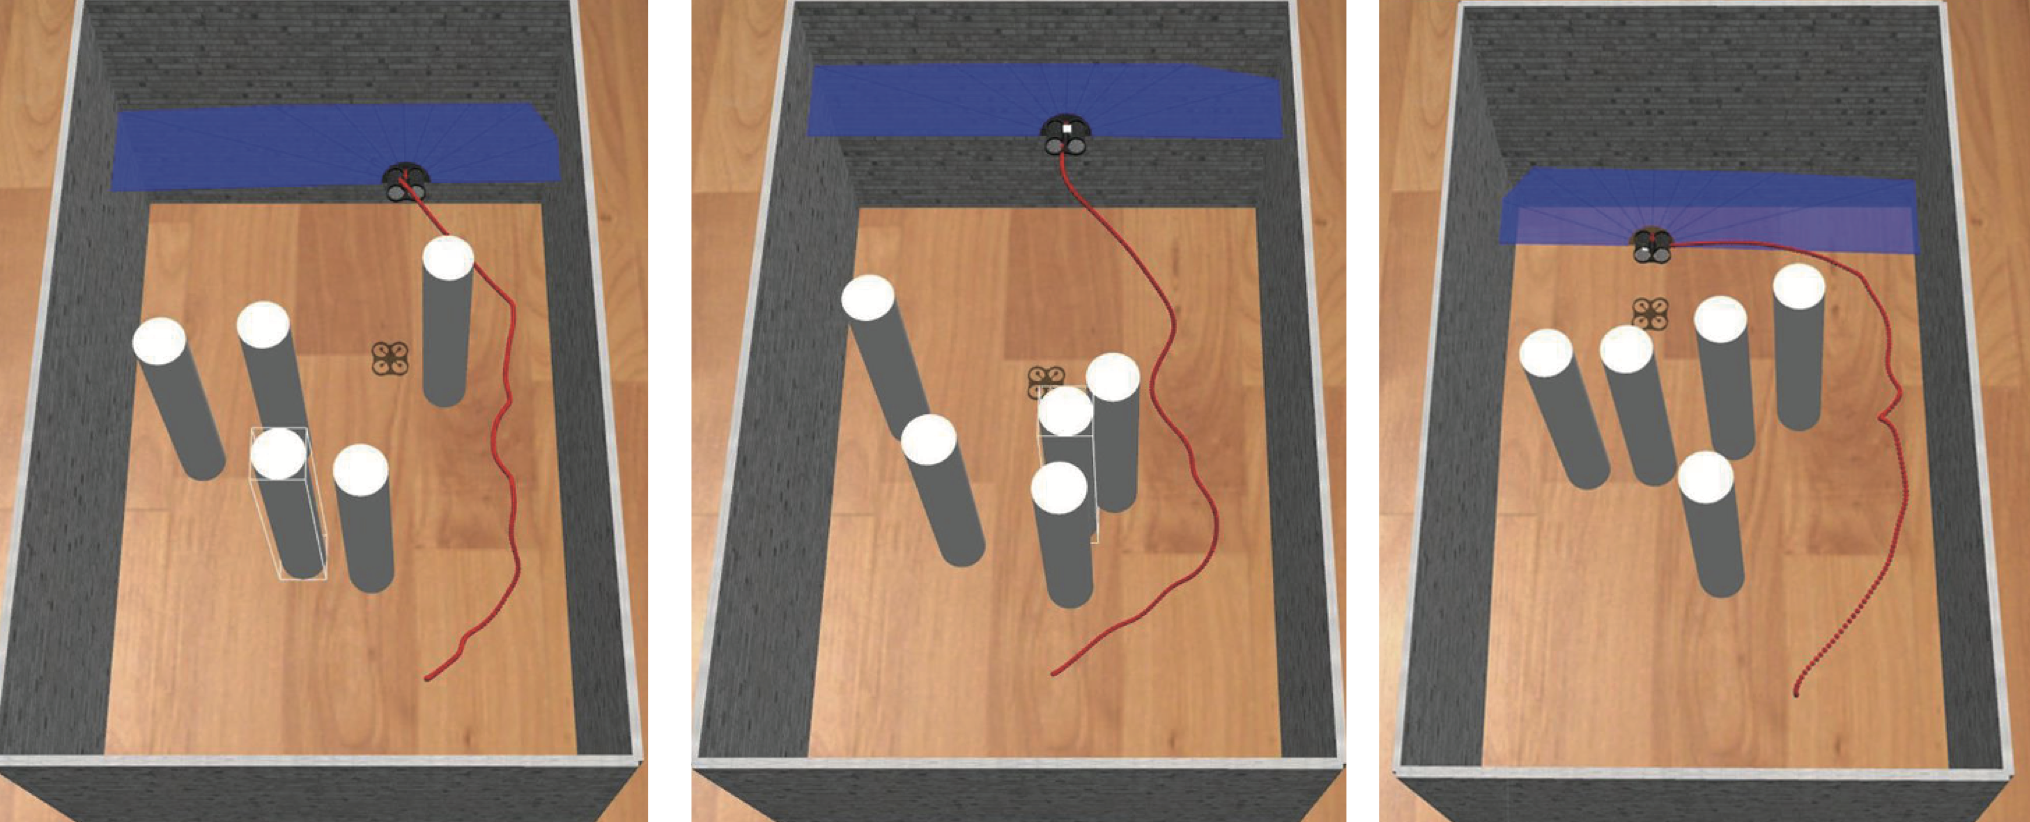
\includegraphics[width=\textwidth]{background/fyp17-sacfd.png}
  \caption{Mapless navigation environment for Soft Actor Critic from Demonstrations}
\label{fig:fyp17-sacfd}
\end{figure}

The reward used 3 cases as shown in Equation.~\ref*{eq:fyp17-sacfd-reward}. 
The final case effectively shows a hieristic was used to increase rewards closer to encourage the agent to rate positions closer to the destination as higher.

\begin{equation}
  r(s_{t}, a_{t}) =
  \begin{cases} 
    r_{arrive} & |x_{t} - g_{t}| < \delta \\
    r_{obstacle} & l_{t} < \epsilon \\
    1-0.1 |x_{t} - g_{t}| & \text{otherwise}
  \end{cases}
  \label{eq:fyp17-sacfd-reward}
\end{equation}

One of the most interesting parts of this particular paper was its effective use of coordinate frames.
Given one of the main aims for agent to learn to aviod the obstacles.
Rather than being provided with a view on the map or locations of the obstacles, observations were provided around the drone, which effectively gave distances to obstacles in each direction around the drone.
This is effectivley measuring everything from a drone coordinate frame.
Within the particular drone perching task, the choice of coordinate frames in more complex, since there are multiple relations between objects that are important to account for.
There is the drone itself, the perching branch and also the tether.
An in particular since the dynamics between the tether and the drone are complex to model in simulation, this is an are where demonstration could be a very useful application.

An interesting observation in this paper is that many reinforcment learning algorithms are trained on a single map.
One of the major aims here was in generalisation and the understanding from measurements for any map rather than "memorizing" a particular map.
Therefore in this environment the positions of the obstacles and destination were randomly assigned in each episode to ensure that generalisation from observations occurred.
One area of note in this particular examples, is the trajectories themselves that this algorithm generate are largely not smooth and could prove complex and non-efficient to actually fly in a real environment.

\todo{improve diagram showing the environment}


\section{Inverse Reinforcement Learning}
% FYP10 Soft Actor-Critic with Inhibitory Networks for Retraining UAV Controllers Faster

%     - FYP10 - Soft Actor-Critic with Inhibitory Networks for Retraining UAV Controllers Faster
%     - FYP18 - Inverse Reinforcement Learning
%     - FYP-15 - Demonstration Guided Reinforcment Learning with Learned Skills